\documentclass{standalone}

\usepackage{tikz}
\newcommand\fl[1]{\texttt{#1}}
\usetikzlibrary{decorations.markings,calc}
\tikzset{->-/.style={postaction=decorate,decoration={markings, mark=at position
#1 with \arrow{latex}}}}

\begin{document}
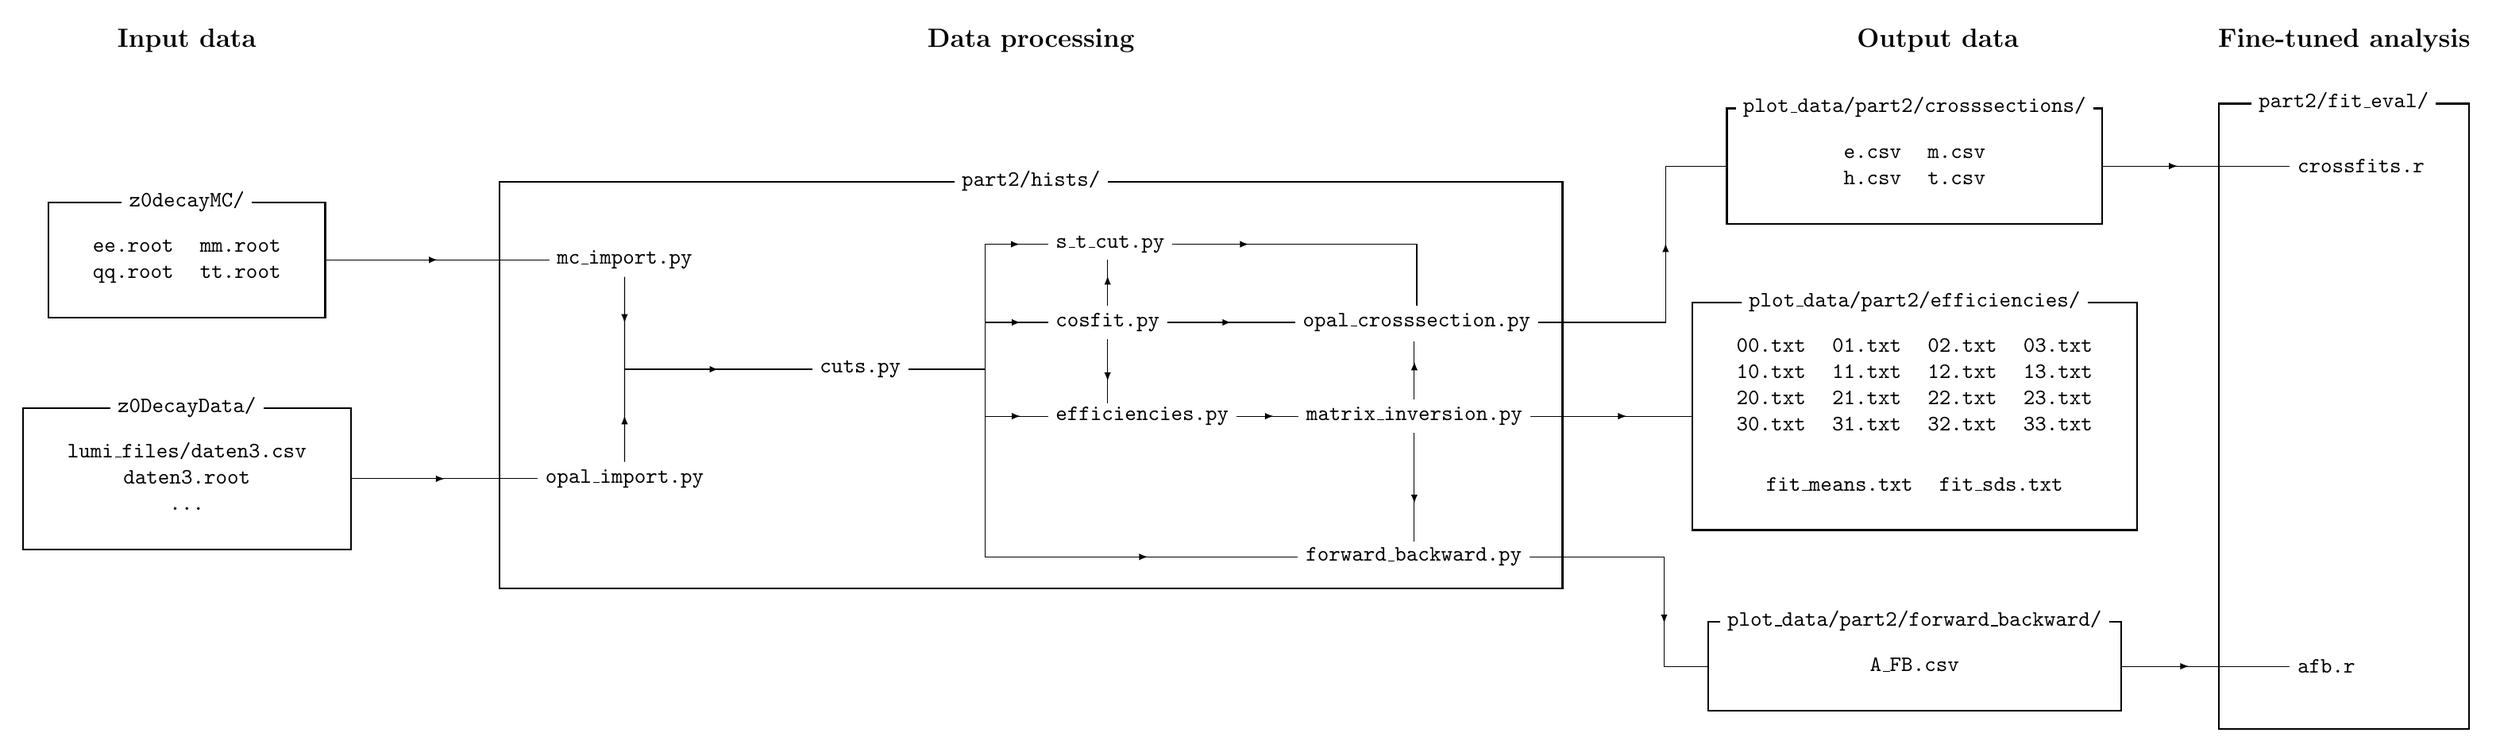
\begin{tikzpicture}
  \node[draw, thick, inner sep=.5cm] at (0, -.5) (in){%
    \begin{tabular}{cc}
      \fl{ee.root} & \fl{mm.root} \\
      \fl{qq.root} & \fl{tt.root} \\
    \end{tabular}
  };
  \node[fill=white] at (in.north) {\fl{z0decayMC/}};

  \node[draw, thick, inner sep=.5cm] at (0, -4) (in2){%
    \begin{tabular}{c}
      \fl{lumi\_files/daten3.csv} \\
      \fl{daten3.root} \\
      \fl{\ldots} \\
    \end{tabular}
  };
  \node[fill=white] at (in2.north) {\fl{z0DecayData/}};

  \node[draw, thick, minimum height=6.5cm, minimum width=17cm, inner sep=.5cm] 
    at (13.5, -2.5) (eval) {};
  \node[fill=white] at (eval.north) {\fl{part2/hists/}};
  \node (mcimport)   at ($(in) +(7, 0)$) {\fl{mc\_import.py}};
  \node (opalimport) at ($(in2)+(7, 0)$) {\fl{opal\_import.py}};
  \draw[->-=.5] (in) -- (mcimport);
  \draw[->-=.5] (in2) -- (opalimport);

  \coordinate (temp) at ($(mcimport)!.5!(opalimport)$);
  \draw[->-=.5] (mcimport)   -- (temp);
  \draw[->-=.5] (opalimport) -- (temp);
  \draw[->-=.5] (temp) --++ (3, 0) node[right] (cuts) {\fl{cuts.py}};
  \draw (cuts) --++ (2, 0) coordinate (temp2);
  \draw[->-=.75] (temp2) |-++ (1, 0.75) node[right] (cosfit) {\fl{cosfit.py}};
  \draw[->-=.75] (temp2) |-++ (1,-0.75) node[right] (efficiencies)
    {\fl{efficiencies.py}};
  \draw[->-=.85] (temp2) |-++ (1, 2) node[right] (stcut)  {\fl{s\_t\_cut.py}};
  \draw[->-=.70] (temp2) |-++ (5,-3) node[right] (forwardbackward)
    {\fl{forward\_backward.py}};
  \draw[->-=.65] (cosfit) --++ (0, 1.0);
  \draw[->-=.65] (cosfit) --++ (0,-1.3);

  \draw[->-=.6] (efficiencies) --++ (2.5, 0) node[right, align=center]
    (matrixinversion)
    {\fl{matrix\_inversion.py}};
  \draw[->-=.65] (matrixinversion) --++ (0, -2);
  \draw[->-=.65] (matrixinversion) --++ (0, 1.2);

  \draw[->-=.5]  (cosfit) --++ (3, 0) node[right] (opalcr)
    {\fl{opal\_crosssection.py}};
  \draw[->-=.25] (stcut) -| (opalcr);


  \node[draw, thick, inner sep=.5cm, minimum width=6cm] at 
    ($(matrixinversion) + (8, 4)$) (out1){%
    \begin{tabular}{cc}
      \fl{e.csv} & \fl{m.csv} \\
      \fl{h.csv} & \fl{t.csv} \\
    \end{tabular}
  };
  \node[fill=white] at (out1.north) {\fl{plot\_data/part2/crosssections/}};

  \node[draw, thick, inner sep=.5cm, minimum width=6cm, align=center]
    at ($(matrixinversion) + (8, 0)$) (out3){%
    \begin{tabular}{cccc}
      \fl{00.txt} & \fl{01.txt} & \fl{02.txt} & \fl{03.txt} \\
      \fl{10.txt} & \fl{11.txt} & \fl{12.txt} & \fl{13.txt} \\
      \fl{20.txt} & \fl{21.txt} & \fl{22.txt} & \fl{23.txt} \\
      \fl{30.txt} & \fl{31.txt} & \fl{32.txt} & \fl{33.txt} \\
    \end{tabular} \\[.5cm]
    \begin{tabular}{cc}
      \fl{fit\_means.txt} & \fl{fit\_sds.txt}  \\
    \end{tabular}
  };
  \node[fill=white] at (out3.north) {\fl{plot\_data/part2/efficiencies/}};

  \node[draw, thick, inner sep=.5cm, minimum width=6.6cm] at
    ($(matrixinversion) + (8, -4)$) (out2){%
    \begin{tabular}{c}
      \fl{A\_FB.csv}
    \end{tabular}
  };
  \node[fill=white] at (out2.north) {\fl{plot\_data/part2/forward\_backward/}};

  \draw[->-=.6] (matrixinversion) -- (out3);
  \draw[->-=.6] (opalcr) 
    -| ($(opalcr)!.5!(out1)$)
    |- (out1);
  \draw[->-=.7] (forwardbackward) 
    -| ($(forwardbackward)!.5!(out2)$)
    |- (out2);

  \draw[->-=.4] (out1) --++ (6, 0) node[right] (r1) {\fl{crossfits.r}};
  \draw[->-=.4] (out2) --++ (6, 0) node[right] (r2) {\fl{afb.r}};

  \node[draw, thick, minimum height=10cm, minimum width=4cm, inner sep=.5cm] 
    at ($(r1)!.5!(r2)$) (r) {};

  \node[fill=white] at (r.north) {\fl{part2/fit\_eval/}};

  \node[font=\large\bfseries] at (0, 3) {Input data};
  \node[font=\large\bfseries] at (13.5, 3) {Data processing};
  \node[font=\large\bfseries] at (28, 3) {Output data};
  \node[font=\large\bfseries] at (34.5, 3) {Fine-tuned analysis};

\end{tikzpicture}
\end{document}
